Le domaine de compression des graphes est un domaine qui a connu une grande évolution vu son importance. Une multitude de méthodes ont été proposées au cours des dernières années. Elles diffèrent l'une de l'autre dans plusieurs points : le type de graphe en entrée, le type de structure en sortie, le type de compression et la technique utilisée pour la compression. En se basant sur ces différences, plusieurs classifications ont été suggérées. Nous allons dans ce qui suit présenter les plus importantes parmi ces classifications.\\

Dans \citep{maneth2015survey}, les auteurs proposent une classification basée tout d'abords sur le type de compression. Ils regroupent les méthodes en deux catégories principales : les méthodes de compression sans perte et les méthodes de compression avec perte. La première catégorie est subdivisée à son tour selon le type de représentation du graphe en sortie : représentation succinte, représentation structurelle ou une représentation sous forme de fichier RDF\newacronym{rdf}{RDF}{Resource Description Framework}\footnote{\gls{rdf} : est un modèle de graphe destiné à décrire de façon formelle les ressources Web et leurs métadonnées, de façon à permettre le traitement automatique de telles descriptions.}. 
Les méthodes donnant une représentation succincte représentent le graphe sous forme d'une chaine de bits succincte irréversible lors de la décompression. La sortie de ces méthodes est ainsi une structure compacte du graphe originale. Parmi les méthodes de cette classe, nous trouvons : Web Framework de Boldi et Vigna \citep{boldi2004webgraph}. La deuxième classe est la représentation structurelle. Contrairement à l'approche précédente, les méthodes de cette classe modifient la structure du graphe initial, sachant que les modifications apportées sont réversibles. La sortie sera donc une structure réduite et non pas compacte de la version initiale. Parmi ces méthodes, nous citons : RePair de Claude et Navarro \citep{claude2010fast}. La dernière classe est la compression  des fichiers \gls{rdf} et qui comporte des méthodes assez récente. Nous trouvons parmi ces techniques : Dcomp de \citep{martinez2012compression} . Les méthodes de compression avec perte quant à elles apportent des modifications irréversibles sur le graphe en supprimant les informations redondantes et le bruit. Comme exemple, nous citons : ASSG de Zhang et al. \citep{zhang2014assg}.\\

Une autre classification a été exposée par Lui et al. dans \citep{liu2018graph} qui classe les méthodes sur trois niveaux. Au premier et deuxième niveaux, les techniques de compression sont regroupées en fonction du type de graphe en entrée selon deux critères : graphe statique ou dynamique et graphe simple ou étiqueté. Pour le troisième niveau, les auteurs catégorisent les méthodes selon la technique de traitement utilisée. Quatre catégories sont définies: les méthodes de regroupement ou d'agrégation, ces méthodes permettent d'agréger de manière récursive un ensemble de nœuds, liens ou carrément un cluster en un super nœud (appelé parfois nœud virtuel), comme exemple de ces techniques, nous trouvons Grass \citep{lefevre2010grass}. Le deuxième type de méthodes englobe les méthodes de compression de bits. Ces méthodes minimisent le nombre de bits nécessaires au stockage du graphe en se basant sur 
\newacronym{mdl}{MDL}{Minimum Description Length} 
le principe de description minimal (\gls{mdl} en Anglais). Elles peuvent être avec ou sans perte. Parmi elles, nous citons LSH-based \citep{khan2014set}. La troisième classe comporte les méthodes de simplification qui suppriment les arêtes les moins importantes selon un certain critère. Parmi ces méthodes, nous trouvons \citep{shen2006visual}. La dernière catégorie est la classe des méthodes basées sur l'influence, les méthodes de cette catégorie décrivent le graphe par les flux d'influence les plus importants ce qui permet de l'analyser plus facilement. Ces méthodes permettent de formuler le problème de compression comme un processus d'optimisation dans lequel la quantité de données liée à l'influence est maintenue en sortie. Parmi ces techniques, nous mentionnons \citep{shi2015vegas}.\\


La dernière classification que nous allons présenter est la classification proposée dans un master de l'année dernière par le binôme : Mlle. Belhocine et Mr. Guermah \citep{master2017}. Cette classification se base sur le principe utilisé dans le processus de compression. Elle regroupe six classes de méthodes : 1) compression basée sur l'ordre des nœuds en exploitant le principe de similarité et de localité du graphe, les méthodes de cette catégorie cherchent à trouver un ordre des nœuds, qui doit répondre à deux propriétés essentielles : la similarité \footnote{ Deux nœuds proches ont tendance à avoir des voisins similaires} et la localité \footnote{ les liens sortants d'un nœud ont tendance à se diriger vers un ensemble
de nœuds qui sont proches.}, cet ordre est ensuite utilisé dans la construction d'une structure de données qui compresse le graphe en entée, comme exemple de ces méthodes, nous trouvons Layered Label Propagation \citep{boldi2011layered} qui utilise l'ordre LLP \footnote{LLP est un algorithme itératif qui produit une séquence d’ordres de nœuds en se basant sur les étiquettes affectées aux clusters après avoir partitionner le graphe initial.} et Recursive Graph Bisection de \citep{dhulipala2016compressing} qui utilise un ordre BP \footnote{BP est un ordre basée sur le problème de bissection de graphes, qui cherche à trouver une meilleure partition des nœuds du graphe tout en minimisant une fonction objectif.}. 2) compression basée sur l'ordre des nœuds en exploitant la linéarisation du graphe, les méthodes de cette classe se basent sur une nouvelle structure de données intitulée structure de données eulérienne, elles sont conçues principalement pour les grands graphes, parmi ces méthodes nous trouvons Neighbor Query Friendly Compression 
\citep{maserrat2012community}. 3) compression basée sur l'étiquetage des nœuds par des intervalles, ces méthodes visent a construire une structure d'index à partir du graphe initial qui permet de répondre aux requêtes de voisinage, parmi ces méthodes nous citons DAGGER \citep{yildirim2012grail}. 4) compression basée sur la structure d'arbre ${K}^{2}$, les méthodes de cette catégorie s'appuient sur la représentation ${K}^{2}$-trees pour compresser le graphe, ces méthodes font l'objet de notre travail et seront détaillées par la suit. 5) compression basée sur l'agrégation des nœuds, ces méthodes sont parmi les méthodes les plus populaires dans le domaine de compression, elles cherchent à compresser le graphe initial en agrégeant un certain nombre de nœuds en un seul nœud appelé super-nœud, cette agrégation se fait selon différentes manières, elle peut être orientée par une fonction objectif représentant l’espace de stockage optimal généralement établie par le principe de la longueur
de description minimale LDM ou par la similarité des caractéristiques des nœuds tels que les
labels et les attributs ou par l’extraction de motifs en utilisant des techniques de pattern mining, cette dernière représente l'une des matières de notre recherche. 6) compression basée sur l'agrégation des liens, contrairement aux techniques précédentes, les méthodes de cette classe visent à compresser le graphe initial en fusionnant certains ensembles de ses liens en un seul liens appelé super-lien, elle est établie selon deux façons, elle est orientée soit par le biais des règles de grammaire, ou bien par l'extraction de motifs que nous allons étudier par la suit.\\

%Après l'étude des méthodes basées sur l'agrégation par extraction de motifs, nous avons constaté que certaines classes ne sont pas bien définies. Les imperfections que nous avons remarqué peuvent être énumérées comme suit : 1) les méthodes d'extraction de motifs englobent certaines méthodes d'agrégation et non pas le contraire, 2) Les méthodes d'extraction de motifs ne sont pas toutes des méthodes agrégatives, nous trouvons parmi elles d'autres méthodes basées sur un vocabulaire. Nous avons donc apporté des modifications sur cette classification. La figure \ref{classif} représente la classification de l'année passé après raffinement où nous avons marqué nos apports en rouge.

Après l'étude des méthodes basées sur l'agrégation par extraction de motifs, nous avons constaté que certaines classes ne sont pas bien définies. Nous avons remarqué que la classification a proposé d'inclure les méthodes basées sur l'extraction de motifs dans deux classes de méthodes qui sont : les méthodes basée sur l'agrégation des liens et les méthodes  basée sur l'agrégation des nœuds, or ce sont les méthodes d'extraction de motifs qui englobent certaines méthodes d'agrégation et non pas le contraire. En effet, notre étude bibliographique a clairement montré que les méthodes de compression de graphe par extraction de motifs ne sont pas toutes des méthodes agrégatives. Nous trouvons, par exemple, certaines de ces méthodes qui donnent en sortie une liste des motifs les plus pertinents du graphe avec une matrice d'erreur sans avoir recours à l'agrégation. Donc nous avons proposé de dissocier la classe des méthodes basées sur extraction de motifs de la classe des méthodes basées sur l'agrégation.
En outre, nous avons considéré, contrairement à la classification précédente, que les méthodes de compression basées sur les règles de grammaire font parties des méthodes de compression par extraction de motifs. Nous justifiant cela par le fait que ces méthodes utilisent l'un des deux principes suivants : 
\begin{enumerate}
\item La transformation la liste d'adjacence en une chaine de caractère et le remplacement, de manière itérative, de la sous-chaine de longueur 2 la plus fréquente en une règle de production.
\item La recherche d'un motif, appelé \textit{digram}\footnote{Un digramme : est sous-graphe composé de deux arêtes ayant un sommet en commun}, satisfaisant une certaine condition et le remplacement toutes ses occurrences par une production dans la grammaire. 
\end{enumerate}
Le fait que les motifs dans le cas de cette classe n'ont pas une structure de sous-graphes connus (clique, étoile, ...) n'empêche pas que le processus appliqué est toujours le même. Nous avons essayer donc de rectifier ses imperfections tout en raffinant davantage les deux classes qui font l'objet de notre Master. 

La classe des méthodes de compression par les arbres k2-trees ne peut être encore raffinée car elles partagent toutes le même principe et diffèrent dans le type de graphe en entrée ou dans le codage en sortie.

Pour la classe des méthodes de compression par extraction de motifs, nous distinguons cinq classes: 1)les méthodes de compression basées vocabulaire faisant appel aux méthodes de clustering, 2) les méthodes de compression basées vocabulaire exploitant les propriétés de la matrice d'adjacence, 3) les méthodes de compression basées agrégation des nœuds des motifs, 4) les méthodes de compression basées agrégation des liens des motifs utilisant des règles de grammaire, 5) les méthodes de compression basées agrégation des liens des motifs faisant appel à des heuristiques de partitionnement de graphes. La première et la deuxième classe se caractérisent par l'ensemble des motifs qui est prédéfini au départ. Cependant, elles se distinguent l'une de l'autre dans le principe de fonctionnement : l'une utilise des méthodes de clustering et de détection de communautés tant dis que l'autre utilise directement la matrice d'adjacence en exploitant ses propriétés. Les trois (03) dernières classes forment l'ensemble des méthodes d'extraction de motifs basées sur l'agrégation de ces derniers. 



 La figure \ref{classif} représente la classification de l'an dernier après raffinement où nous avons marqué nos apports et nos modifications en rouge.

 \begin{figure}[H]
		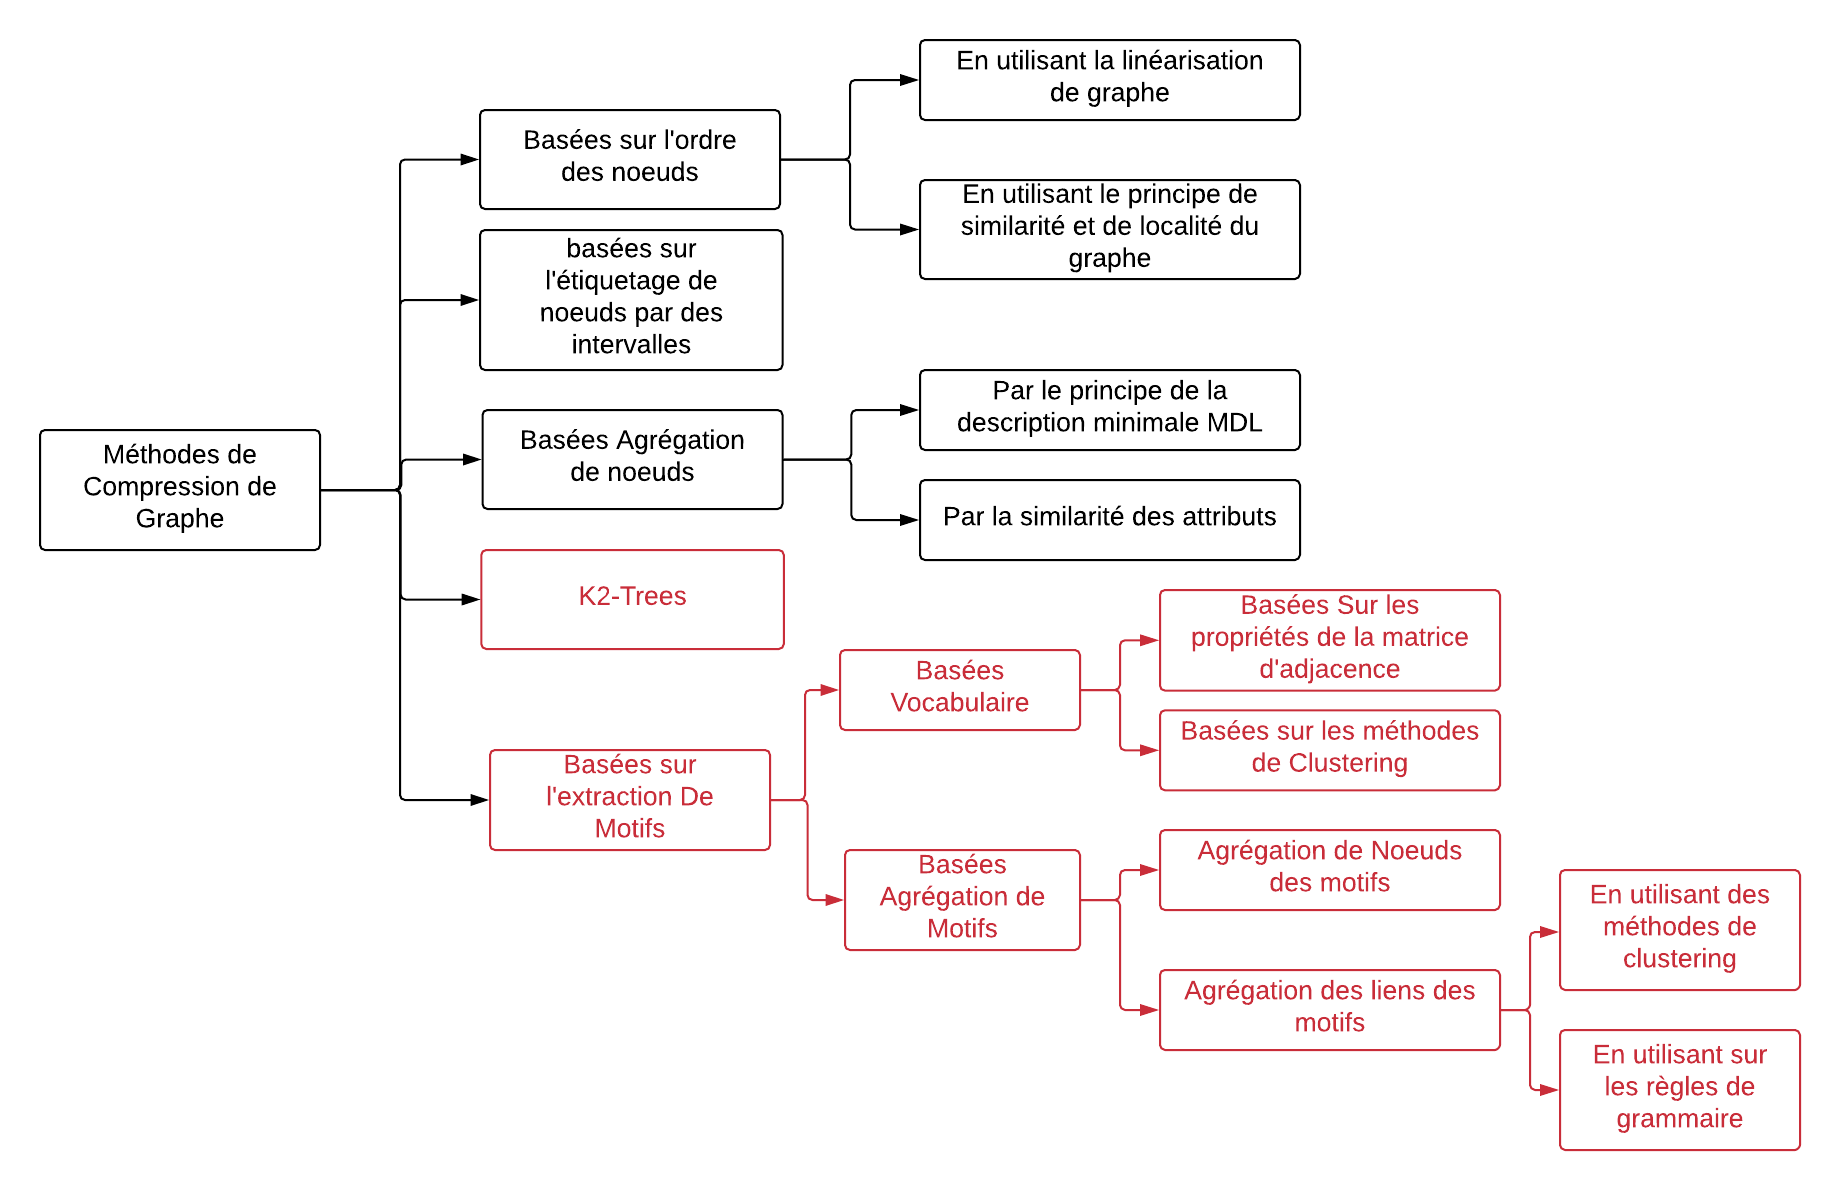
\includegraphics[scale=0.55]{./ressources/image/classif.png}
		\caption{Classification proposées des méthodes de compression}
		\label{classif}
	\end{figure}





